% -*- TeX:de -*-
\NeedsTeXFormat{LaTeX2e}
\documentclass[12pt,a4paper]{article}
\usepackage[german]{babel} % german text
\usepackage[DIV12]{typearea} % size of printable area
\usepackage[T1]{fontenc} % font encoding
%\usepackage[latin1]{inputenc} % most likely on Windows
\usepackage[utf8]{inputenc} % probably on Linux
\usepackage{multicol}

% PLOTTING
\usepackage{pgfplots} 
\usepackage{pgfplotstable}
\usepackage{url}
\usepackage{graphicx} % to include images
\usepackage{tikz}
\usepackage{subfigure} % for creating subfigures
\usepackage{amsmath} % a bunch of symbols
\usepackage{amssymb} % even more symbols
\usepackage{booktabs} % pretty tables
\usepackage{makecell} % multi row table heading

% a floating environment for circuits
\usepackage{float}
\usepackage{caption}

%\newfloat{circuit}{tbph}{circuits}
%\floatname{circuit}{Schaltplan}

% a floating environment for diagrams
%\newfloat{diagram}{tbph}{diagrams}
%\floatname{diagram}{Diagramm}

\selectlanguage{german} % use german

\begin{document}

%%%%%%% DECKBLATT %%%%%%%
\thispagestyle{empty}
			\begin{center}
			\Large{Fakultät für Physik}\\
			\end{center}
\begin{verbatim}


\end{verbatim}
							%Eintrag des Wintersemesters
			\begin{center}
			\textbf{\LARGE SS 14}
			\end{center}
\begin{verbatim}


\end{verbatim}
			\begin{center}
			\textbf{\LARGE{Physikalisches Praktikum\\ für das Bachelorstudium}}
			\end{center}
\begin{verbatim}




\end{verbatim}

			\begin{center}
			\textbf{\LARGE{PROTOKOLL}}
			\end{center}
			
\begin{verbatim}

\end{verbatim}

			\begin{flushleft}
			\textbf{\Large{Experiment (Nr., Titel): PS9 - Heißluftmotor - Stirlingprozess}}\\
							%Experiment Nr. und Titel statt den Punkten eintragen
			\LARGE{PS09 }	
			\end{flushleft}

\begin{verbatim}

\end{verbatim}	
							%Eintragen des Abgabedatums, oder des Erstelldatums des Protokolls
			\begin{flushleft}
			\textbf{\Large{Datum:}} \Large{10.04.2014}
			\end{flushleft}
			
\begin{verbatim}
\end{verbatim}
							%Namen der Protokollschreiber
		\begin{flushleft}
			\textbf{\Large{Namen:}} \Large{Patrick Braun, Johannes Kurz}
			\end{flushleft}

\begin{verbatim}


\end{verbatim}
							%Kurstag und Gruppennummer, zb. Fr/5
			\begin{flushleft}
			\textbf{\Large{Kurstag/Gruppe:}} \Large{DO/4}
			\end{flushleft}

\begin{verbatim}

\end{verbatim}
							%Name des Betreuers, das Praktikum betreute.
			\begin{flushleft}
			\LARGE{\textbf{Betreuer:}}	\Large{Johanna Akbarzadeh}	
			\end{flushleft}

%%%%%%% DECKBLATT ENDE %%%%%%%
\pagebreak
\setlength{\columnsep}{20pt}
\begin{multicols}{2}

%%%%%%%%%%%%%%%%%%%%%%%%%%%%%%%%%%%%%%%%%%%%%%%%

%\begin{figure}[H]
%	\centering
%	\includegraphics[scale=0.35]{./data/beugung.png}
%	\caption{Beugungsmuster Einzelspalt (echtes Foto; schwarz durch weiß ersetzt)}
%	\label{fig:beugungsmuster}
%\end{figure}


%\begin{figure}[H]
%	\centering
%	\pgfplotstabletypeset[
%			columns={abstand, n},
%			col sep=&,
%			columns/abstand/.style={precision=2, zerofill, column name=\makecell{$Abstand$\\$(\pm 0.05)[mm]$} }, 
%			columns/n/.style={column name=\makecell{$n$\\$(Ordnung)$}, precision=0},
%			every head row/.style={before row=\hline,after row=\hline\hline},
%			every last row/.style={after row=\hline},
%			every first column/.style={column type/.add={|}{} },
%			every last column/.style={column type/.add={}{|} }
%			]{
%			abstand & n
%			12.9 & 1
%			24.45 & 2
%			37.40 & 3
%			49.35& 4
%			62.45 & 5
%			74.45 & 6
%			87.45 & 7
%			100.25 & 8
%			
%			}
%	\caption{Messwerte Einzelspalt}
%	\label{tab:werte_einzelspalt}
%\end{figure}


%%%%%%%%%%%%%%%%%%%%%%%%%%%%%%%%%%%%%%%%%%%%%%%%
%%%%%%%%%%%%%%%%%%%%%%%%%%%%%%%%%%%%%%%%%%%%%%%%
\noindent Im Folgenden werden unterschiedliche Anwendungen einer Stirling-Maschine untersucht. Als Wärmekraftmaschine auf Grundlage des Carnotprozesses und in abgeänderter Form als Kältemaschine.\\
Als wichtigstes Maß eines Motors errechnen wir den Wirkungsgrad jeder Anwendung.


\section{Der Heißluftmotor als Wärmekraftmaschine}
In diesem Teil des Experiments bestimmen wir den Wirkungsgrad eines Stirlingmotors über die Leistung welche zugeführt wird und abgenommen werden kann. Zu erst bestimmen wir den idealen Wirkungsgrad, danach den realen Wirkungsgrad und zu Letzt den Wirkungsgrad des Motors.

\subsection{Grundlagen}
Für die Berechnungen benötigen wir folgende Formeln ([1] (pp. 6-8)):\\
$$\eta{ideal} = \frac{T_1 - T_2}{T_1}$$
Bei diesem idealen Verhalten geht keine Energie über Reibung oder Abstrahlung verloren.
$$\eta_{real} = \frac{P_{Motor}}{P_{Zugeführt}}$$
Der reale Wirkungsgrad ist der aussagekräftigste. Dabei wird die aufgewendete Leistung der abnehmbaren Leistung gegenüber gestellt.
$$\eta_{Motor} = \frac{P_{Motor}}{\oint p dV * f}$$
Den Wirkungsgrad des Motors erhalten wir durch die Leistung des Motors (jeweilig beschrieben durch Abnehmer) gebrochen durch die Leistung beschrieben durch die eingeschlossene Fläche im Carnotprozess (entspricht der Energie) mal die Frequenz. 

\subsection{Versuchsaufbau}
In diesem Experiment wird ein bereits aufgebauter Stirlingmotor mit einer Heizspindel und einer Kühlung betrieben (Abbildung  \ref{fig:stirlingMotor_3D}). Als Grundlage dient der bereits beschriebene Carnotprozess. \\
\\
Das Volumen des Zylinder ergibt sich durch (auf den Nullpunkt angepasst):\\
$Volumen = Weg (\pm 0.08mm) * Fläche 28.3 + 195 = $\\ %%%% TODO ergebnis %%%%%
Der Bereich für den Druck
$Druck (-2000 - +2000 \pm 2) hPa$\\

%%%%% TODO AUSTAUSCHEN AUF 3D %%%%%
\begin{figure}[H]
	\centering
	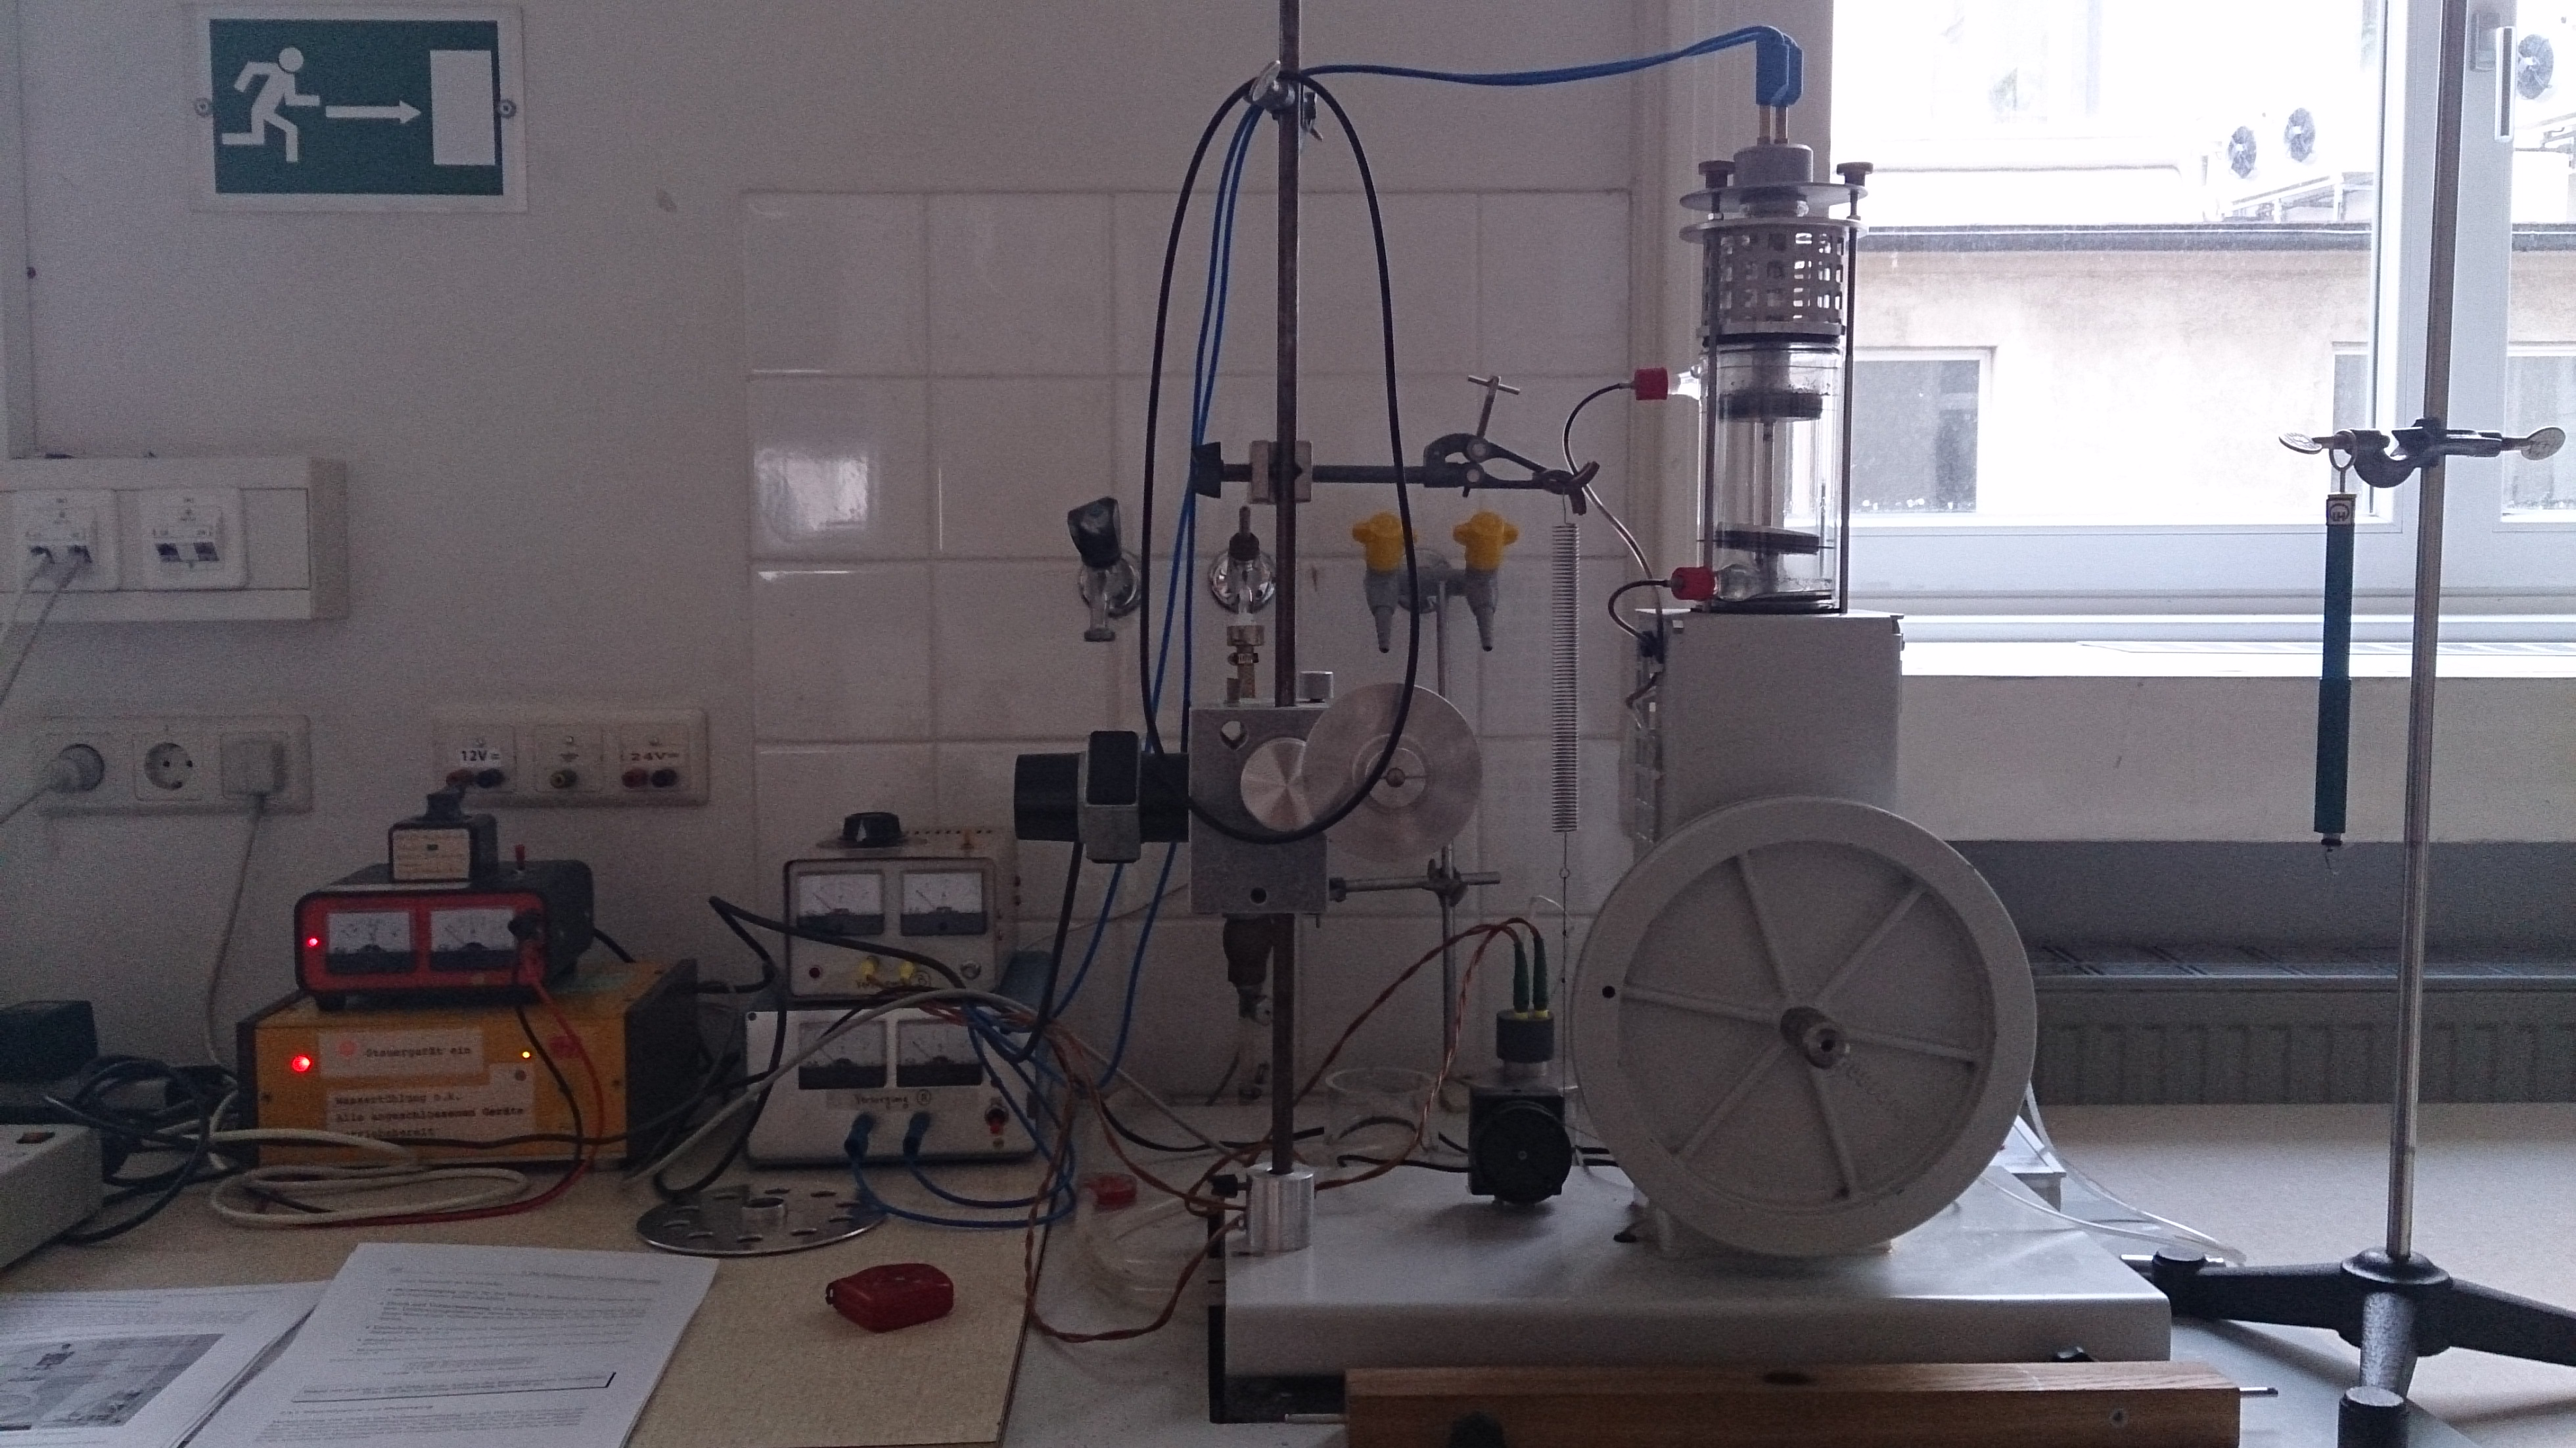
\includegraphics[scale=0.05]{./data/3D-Model_Images/DSC_0083.JPG}
	\caption{Versuchsaufbau als 3D Modell}
	\label{fig:stirlingMotor_3D}
\end{figure}

\subsection{Resultate}

Unbelastet:\\
$A_1 = 37130 hPa*cm^3$\\
$A_2 = 38140 hPa*cm^3$\\
$f_2 = \frac{25.32}{3} Hz$\\
$A_3 = 37530 hPa *cm^3$\\
$f_3 = \frac{37.82}{5} Hz$\\
$A_4 = 36660 hPa * cm^3$\\
$f_4 = \frac{25.28}{3} Hz$\\
$A_5 = 37000 hPa * cm^3$\\
$f_5 = \frac{76.18}{10}$\\
\\
$A_6 = 38720  hPa * cm^3$\\
$A_7 = 37250  hPa * cm^3$\\
$f_{6-1} = 7.77 Hz$\\
$f_{6-2 / 7} = 15.49 / 2 Hz$\\
\\
Belastet:\\
$r = (25.0 \pm 0.2)cm$\\
$F_1 = (1 \pm 0.05)N$\\
$f_1 = 54 / 10Hz$\\
$f_2 = 55 / 10Hz$\\
\\
Strom: $(20 \pm 1) A$\\
Spannung: $(14 \pm 0.5) V$\\

\subsection{Diskussion}




%%%%%%%%%%%%%%%%%%%%%%%%%%%%%%%%%%%%%%%%%%%%%%%%
%%%%%%%%%%%%%%%%%%%%%%%%%%%%%%%%%%%%%%%%%%%%%%%%
\section{Die Stirling-Maschine als Kältemaschine}

\subsection{Grundlagen}


\subsection{Resultate}

Zugeführte Leistung:\\
$230V * (0.36 \pm 0.03) A$\\
Temperatur:\\ 
$T_{unten} = (5.2 \pm 0.1)^{\circ}C$\\
$T_{oben} = (6.0 \pm 0.1)^{\circ}C$\\

Kühlung:\\ 
$U_{unten} = (8.0 \pm 0.5)V$\\
$A_{unten} = (1.7 \pm 0.1)A$\\
$U_{oben} = (8.5 \pm 0.5)V$\\
$A_{oben} = (1.8 \pm 0.1)A$\\

Frequenz:\\
$f = \frac{50.6}{10} Hz$\\

\subsection{Diskussion}


\section{Quellen}
$[1]$ Anleitung, \url{http://www.univie.ac.at/anfpra/neu1/ps/ps9/PS9.pdf}\\

\end{multicols}



\end{document}